\section{Seleção de Atributos}\label{sec:fs} 

A seleção de atributos (\textit{feature selection} (FS))\footnote{Este trabalho utilizará os termos em português e inglês indistintamente.} é uma técnica de pré-processamento amplamente utilizada em aprendizado de máquina (AM), particularmente em conjuntos de dados de alta dimensionalidade \cite{Dhal2022,10.1007/978-3-031-23092-9_12,BARBIERI2024123667}. Seu objetivo consiste em identificar um subconjunto de atributos relevantes a partir do conjunto original, buscando, quando possível, reduzir a redundância entre eles, preservar ou melhorar o desempenho preditivo e reduzir a complexidade dos modelos \cite{Theng2024,Emmoh2024}.

No contexto da classificação associativa, conforme discutido na Seção~\ref{sec:ca}, a redução do número de atributos pode contribuir para diminuir o espaço de busca de regras e a complexidade dos classificadores induzidos. Dessa forma, a aplicação de métodos de FS pode proporcionar diferentes benefícios, entre os quais se destacam:
%%%%%%%%%%%%%%%%%%%%%%%%
\begin{itemize}
    \item \textbf{redução da complexidade e do custo computacional}: a diminuição do número de atributos pode reduzir o espaço de busca e o tempo de treinamento dos algoritmos \cite{Theng2024};

    \item \textbf{melhoria do desempenho e redução do risco de \textit{overfitting}}: a remoção de atributos ruidosos ou irrelevantes pode favorecer a capacidade de generalização dos modelos \cite{Dhal2022};

    \item \textbf{aumento da interpretabilidade e apoio à descoberta de conhecimento}: a utilização de um subconjunto menor de atributos pode facilitar a compreensão dos modelos e a identificação de características relevantes para o problema \cite{Dhal2022,KHAIRE20221060}.
\end{itemize}
%%%%%%%%%%%%%%%%%%%%%%%%

Três são as principais abordagens existentes para realização de FS, a saber \cite{Tan2020,Theng2024}: \textbf{filtro}, \textbf{\textit{embedded}} e \textbf{\textit{wrapper}}. A escolha da abordagem de FS é um ponto crítico, pois ela influencia diretamente a estabilidade do subconjunto de atributos selecionados e o desempenho final do modelo \cite{KHAIRE20221060,BARBIERI2024123667}. Em geral tem-se que:
\begin{itemize}
    \item \textbf{filtro}: constitui a abordagem mais simples e computacionalmente eficiente para a seleção de atributos. Os métodos existentes são independentes do algoritmo de AM que será utilizado \cite{Dhal2022,10.1007/978-3-031-23092-9_12,Theng2024,EBRAHIMIWARKIANI2025129372};
    
    \item \textbf{\textit{wrapper}}: utiliza um algoritmo de AM como mecanismo de avaliação de diferentes subconjuntos de atributos, sendo, portanto, dependente de um algoritmo base. Essa abordagem envolve a indução de múltiplos modelos, o que a torna mais custosa computacionalmente \cite{Theng2024};
    
    \item \textbf{\textit{embedded}}: realiza a seleção de atributos durante o processo de indução do modelo, sendo também dependente do algoritmo utilizado \cite{bashir2022novel,Theng2024}. Nessa abordagem, a relevância dos atributos é incorporada ao mecanismo de treinamento do modelo, como ocorre em árvores de decisão, métodos baseados em regularização e \textit{ensembles} de árvores. Em geral, métodos \textit{embedded} apresentam menor custo computacional que abordagens \textit{wrapper}, pois a seleção é integrada ao treinamento do modelo, embora os subconjuntos obtidos tendam a ser mais dependentes do algoritmo empregado.
\end{itemize}

Neste trabalho, são utilizados métodos de filtro como componentes do EFS4AC, devido à sua independência em relação ao algoritmo de classificação e à sua eficiência computacional. Esses métodos avaliam a relevância dos atributos por meio de critérios estatísticos, informacionais ou de dependência, sem utilizar diretamente o desempenho do classificador como função de avaliação \cite{SolorioFernandez2020,Bouchlaghem2022,Theng2024}.

Em abordagens baseadas em \textit{ranking}, os atributos recebem pontuações ou posições de acordo com o critério adotado. A partir dessa ordenação, um subconjunto pode ser definido mediante um limiar (\textit{threshold}) ou pela seleção de um número predefinido de atributos \cite{geng2007feature,jovic2015review,Theng2024}. Entretanto, a definição do subconjunto final constitui uma decisão adicional, uma vez que o \textit{ranking}, isoladamente, não determina quantos atributos devem ser selecionados.

Os métodos de filtro podem ser classificados em \textbf{univariados} e \textbf{multivariados} \cite{SolorioFernandez2020,Theng2024}. Os métodos univariados avaliam cada atributo individualmente, sem considerar explicitamente suas relações com os demais atributos. Já os métodos multivariados consideram relações entre atributos durante o processo de seleção, podendo incorporar critérios de redundância, dependência e interação \cite{SolorioFernandez2020,Dhal2022,Theng2024}.

Entre as principais vantagens dos métodos de filtro destacam-se a eficiência computacional e a independência em relação ao algoritmo de classificação, características que favorecem sua utilização em diferentes conjuntos de dados e modelos preditivos \cite{Dhal2022,Theng2024}. Por outro lado, os métodos univariados apresentam limitações na identificação de redundâncias e interações entre atributos, enquanto os métodos multivariados podem apresentar maior custo computacional. Além disso, diferentes critérios de avaliação podem produzir ordenações distintas dos atributos, e a escolha do ponto de corte pode influenciar a qualidade do subconjunto selecionado \cite{KHAIRE20221060,Theng2024}. Essa diversidade de critérios e resultados constitui uma das motivações para a combinação de diferentes métodos de seleção de atributos, conforme discutido na próxima subseção.

%%%%%%%%%%%%%%%%%%%%%
\subsection{\textit{Ensemble Feature Selection}}
\label{subsec:efs}

O \textit{Ensemble Feature Selection} (EFS) estende o princípio de aprendizado por \textit{ensemble} ao problema de seleção de atributos, combinando os resultados produzidos por múltiplos seletores-base para obter uma avaliação conjunta da relevância dos atributos \cite{bolon2019ensembles,salman2026review}. A motivação para o uso de EFS decorre do fato de que diferentes métodos de FS podem avaliar os atributos segundo critérios distintos e, consequentemente, produzir diferentes \textit{rankings} ou subconjuntos de atributos. Assim, em vez de depender exclusivamente do resultado de um único seletor, um \textit{ensemble} combina múltiplas avaliações com o objetivo de obter uma solução consensual e reduzir a variabilidade do processo de seleção, favorecendo maior robustez e estabilidade \cite{bolon2019ensembles,salman2026review}.

Diferentemente das abordagens filtro, \textit{wrapper} e \textit{embedded}, que caracterizam a forma como os atributos são avaliados e selecionados, o EFS constitui uma estratégia de combinação de múltiplos métodos de FS. Dessa forma, um EFS pode ser composto por seletores pertencentes a uma mesma abordagem ou a diferentes abordagens, combinando, por exemplo, métodos filtro, \textit{wrapper} e \textit{embedded}.

A diversidade entre os componentes de um EFS pode ser introduzida, principalmente, por meio de duas estratégias \cite{bolon2019ensembles}. Nos \textit{ensembles} homogêneos, um mesmo método de FS é aplicado sob diferentes condições, como diferentes amostras do conjunto de treinamento ou configurações do método, produzindo resultados que são posteriormente combinados. Nos \textit{ensembles} heterogêneos, por sua vez, diferentes métodos de FS são aplicados sobre o mesmo conjunto de dados, permitindo que critérios distintos de avaliação dos atributos contribuam para o resultado final. A Figura~\ref{fig:efs_homogeneo_heterogeneo} ilustra essas duas estratégias. Na Figura~\ref{fig:efs_homogeneo_heterogeneo}, $R_1,\ldots,R_k$ representam os \textit{rankings} produzidos pelo mesmo seletor sob diferentes condições no EFS homogêneo, enquanto $R_1,\ldots,R_m$ representam os \textit{rankings} obtidos por diferentes seletores no EFS heterogêneo. Em ambos os casos, os resultados individuais são encaminhados a uma estratégia de agregação, responsável por produzir uma representação consensual da importância dos atributos.

%%%%%%%%%%%%%%
\begin{figure}[htb]
    \centering
    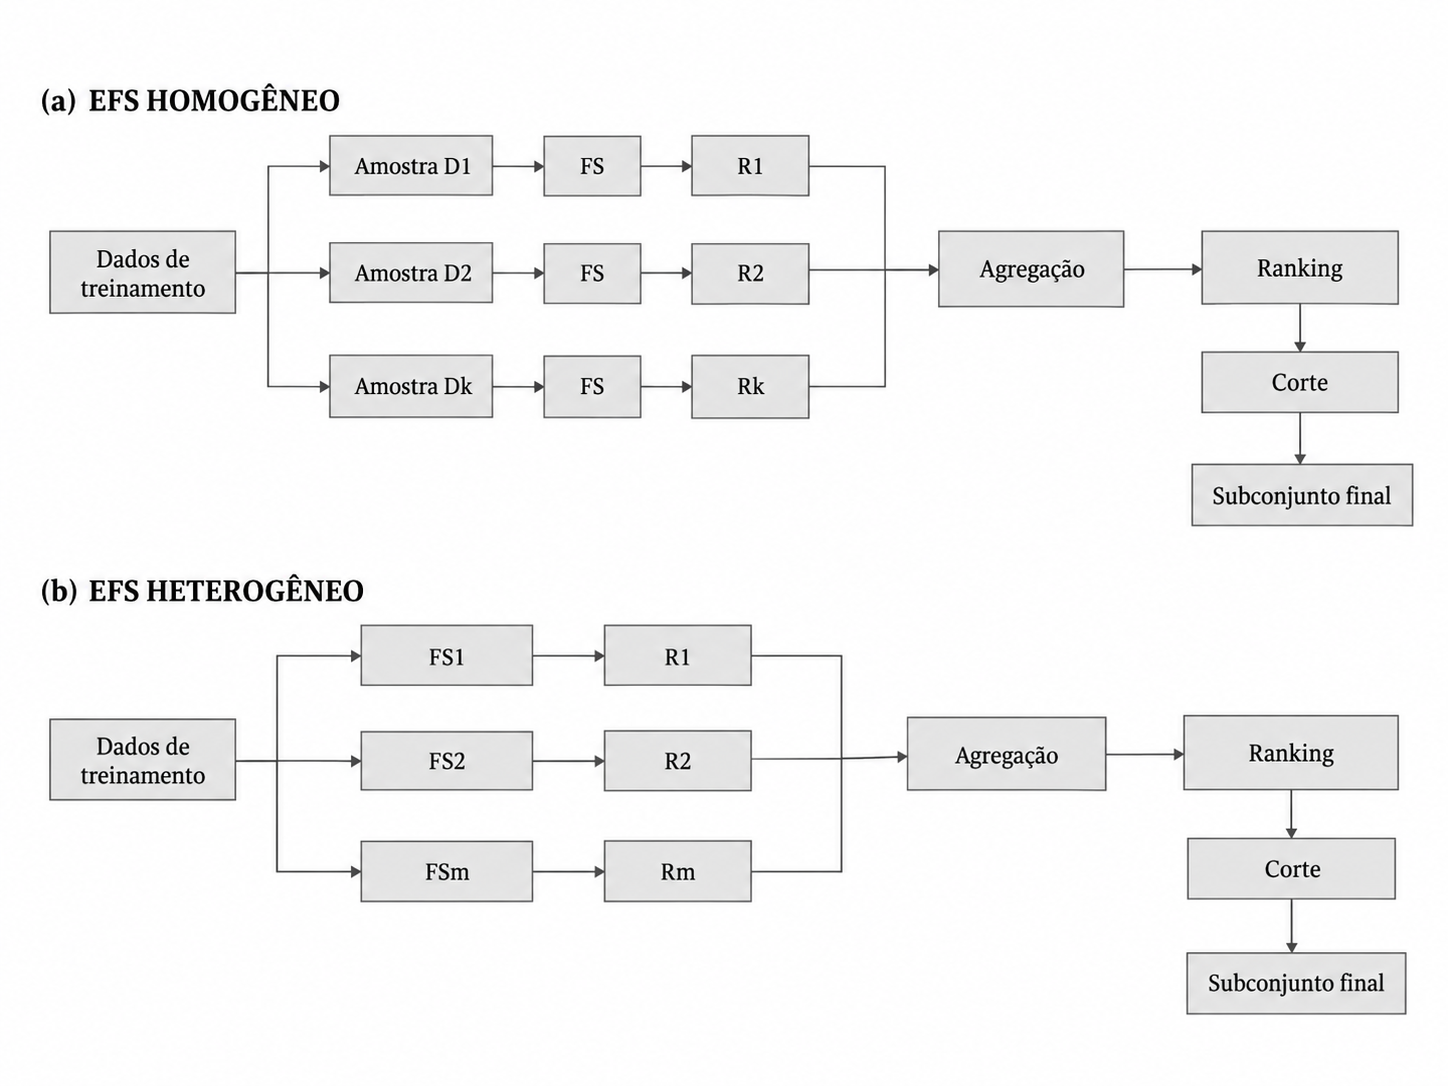
\includegraphics[width=\textwidth]
    {figuras/efs_homogeneo_heterogeneo.png}
    \caption{Estruturas gerais de \textit{Ensemble Feature Selection} homogêneo e heterogêneo. Elaborado pelo autor com base em \citeonline{bolon2019ensembles}.}
    \label{fig:efs_homogeneo_heterogeneo}
\end{figure}
%%%%%%%%%%%%%%

A forma de agregação depende do tipo de saída fornecida pelos seletores-base. Quando os métodos produzem subconjuntos de atributos, esses resultados podem ser combinados diretamente por estratégias de consenso. Quando produzem rankings ou pontuações (scores), diferentes métodos de agregação podem ser utilizados para gerar uma avaliação global da importância dos atributos \cite{bolon2019ensembles}. Nesse segundo caso, torna-se necessária uma etapa adicional de definição do subconjunto final (\textit{thresholding}), responsável por converter a avaliação agregada em um conjunto de atributos selecionados.

Assim, a construção de um EFS envolve diferentes decisões metodológicas, incluindo a composição do conjunto de seletores, a geração de diversidade entre seus componentes, a estratégia de agregação dos resultados individuais e o critério empregado para determinar o subconjunto final de atributos. Essas decisões podem influenciar propriedades importantes do processo de seleção, como estabilidade, robustez e dimensionalidade do subconjunto obtido, bem como o desempenho dos modelos induzidos.
